\section{Background on Xamarin}
\label{section:background}

Xamarin allows the development of native cross-platform mobile apps while
aiming to maximize code-reuse across platforms. Developers using Xamarin target
their apps to its home platform, Windows Phone, and can re-use much of the same
code to build native apps for iOS, Android, and Mac. In this section, we
discuss the structure of a cross-platform app written using Xamarin, and
discuss the techniques that Xamarin uses to allow app logic and data storage
code to be written once and reused across platforms.

A developer using Xamarin can build apps in C\#, using features such as
generics, Linq and the parallel task library. The developer splits the app into
two logical pieces (\figref{figure:appstruct}): \textit{the application core},
which encodes the business logic, and contains code that is common across all
platforms, and \textit{user interface (UI)}, which is written for each platform
and uses the native UI features of that platform, \eg~buttons, widgets, and the
overall look and feel of the specific platform. The developer implements the UI
layer in C\# as well, using native UI design tools such as
\code{Android.Views}, \code{MonoTouch.UIKit} for iOS, and XAML, Silverlight and
Metro APIs for Windows Phone. Xamarin is built atop the Mono \code{.NET}
framework~\cite{mono}, which provides the core cross-platform implementation of
Microsoft's \code{.NET} framework. C\# source code can be compiled with
Xamarin's compiler to produce a native iOS app, or an Android app with
integrated \code{.NET} runtime support. In this case, the C\# code is compiled
to an intermediate language, and packaged with MonoVM configured for
just-in-time compilation on Android.

Xamarin aims to provide support to developers to minimize the amount of
platform-specific code that is needed to port an app across platforms. Some
platform-dependent code is unavoidable, \eg~the UI code shown in
\figref{figure:appstruct}, but there are ongoing efforts such as
\code{Xamarin.Forms} to even minimize the amount of platform-dependent UI code.
However, Xamarin provides extensive support to allow the application core to be
written once and used across multiple platforms, with as little
platform-dependent code as possible. 

\begin{figure}[t!]
\centering
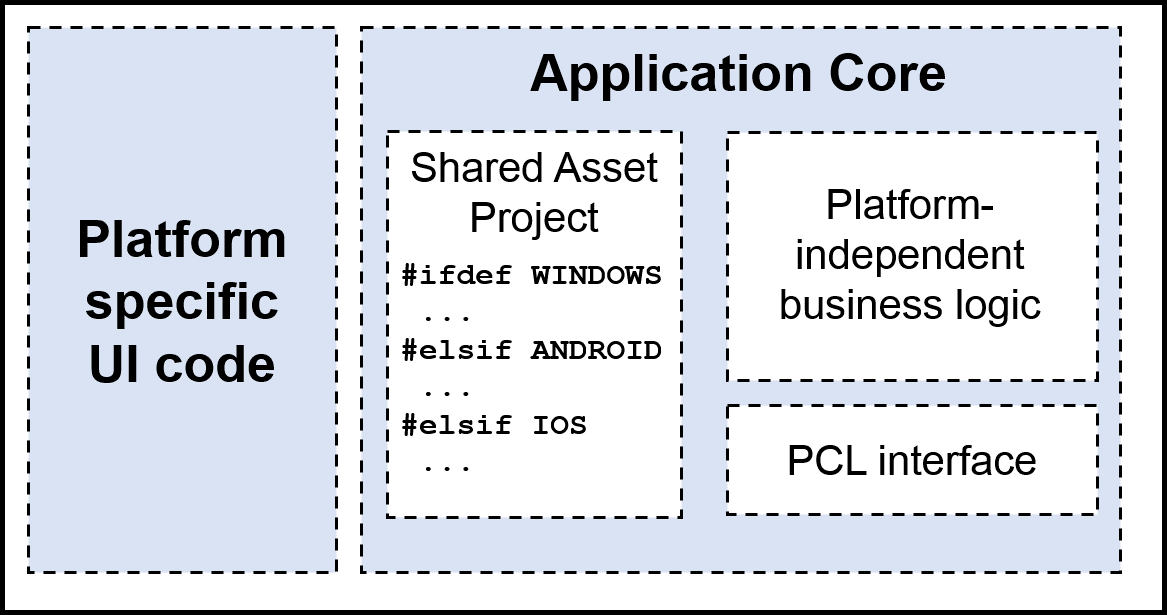
\includegraphics[keepaspectratio=true,width=0.45\textwidth]{figures/appstruct.png}
\mycaption{Structure of a cross-platform app written using Xamarin.}
{\label{figure:appstruct}}
\end{figure}

To achieve this goal, Xamarin supports \textit{portable class libraries}
(PCLs), a technology originally developed by Microsoft. On Visual Studio and
other Microsoft environments, a PCL is a special type of a project that allows
developers to write code and produce libraries that can be shared across
multiple platforms, such as iOS, Android, and Windows Phone. To support this,
PCLs export an interface of methods and properties that are portable across
platforms, and developers program to this interface. PCL provides forwarding
stubs that ensures that calls to methods or property accesses are routed to the
correct underlying platform libraries at runtime. The developer of the PCL
typically identifies the interface by choosing a set of target platforms that
the PCL will support. Because different platforms provide implementations of
differing subsets of the base \code{.NET} class library, the PCL interface is
typically restricted to the common \code{.NET} functionality that is supported
by all the target platforms. 

However, apps may need to use functionality that is outside of the PCL
interface. For example, suppose that an app wishes to access the camera, but
the PCL interface does not support this functionality. In this case, the app
developer has two options. He can create platform-dependent code (akin to the
UI code) containing this functionality, or instead write this code as
\textit{shared asset projects}. This method is used when the developer wishes to
write platform-dependent code, but share the code across multiple platforms. To
do so, shared asset projects usually define platform-dependent code with
compiler or pre-processor directives (\eg~\code{\#ifdef}s) to allow the code to
be written once and compiled for all the desired target platforms. Naturally,
the goal of projects such as Xamarin is to increase the coverage provided by
their PCLs, so as to minimize the amount of code that must be written as shared
asset projects.

% \todo{How many methods supported in Xamarin's PCLs? What fraction of the .NET
% API still not supported?}

In this paper, we are primarily concerned with testing the functionality of the
libraries on Xamarin that provide support for platform-independent app code.
Therefore, the test cases generated by \tool\ only target the PCL interface. We
do not address cross-platform consistency issues related to the UI.

% What are PCLs? How complex are they? What is the total size of Xamarin,
% mono and the PCLs? What does the bug DB say about bugs in various components?






